\chapter{イジング相関、平均場、自発磁化}

\lectureoverview{一次元イジング鎖は、サイトスピンを結合変数に置き換えることで厳密に解くことができる。この変数変換により分配関数は積の形になり、有限温度における相関がすべて指数的に減衰することが示される。高次元の格子は、各スピンが多数の隣接スピンから情報を受け取るため、振る舞いが異なる。それらの複合的な影響を平均場として扱うと、自己無撞着方程式、平均場臨界温度、および任意に小さな外部場がいかにして一方の磁化相を選択するかについての正確な記述が得られる。}

\section{イジングが実際に発見したこと}

歴史的な点は正確に述べられるべきである。エルンスト・イジングはヴィルヘルム・レンツから与えられた一次元模型を解き、有限温度での相転移が存在しないことを正しく見出した。行き過ぎであったのは、同じ結論がすべての次元で成り立つはずだという推論である。それは成り立たない。二次元模型にはすでに秩序化した低温相が存在する。

高次元における厳密解は、現在の目的にはあまりに野心的である。各スピンが多数の隣接スピンを持つ場合に転移を明らかにするには、物理的に透明な近似で十分であろう。しかし、その近似を行う前に、一次元鎖を厳密に解いておく価値がある。厳密な一次元の答えと高次元近似との対比により、一次元に欠けている機構が特定される。

ここでの相転移は、既存の選好が徐々に強まること以上のものを意味する。温度が臨界値を横切ると、平衡状態は新たな巨視的性質を獲得する。すなわち、試料を配向させるために用いた外部場を取り除いた後でも、非零の磁化が持続しうるのである。したがって計算は、二つの別個の問いに答えなければならない。遠くのスピンは選ばれたスピンの配向を記憶しているか、そして無限小の場が任意に大きな試料を組織化できるか。

\section{再利用可能な構成要素としての一つのスピン}

二状態変数
\begin{equation}
\sigma=\pm1,
\end{equation}
をとり、エネルギー規約
\begin{equation}
E(\sigma)=-J\sigma,
\qquad J>0.
\end{equation}
を選ぶ。このとき状態\(\sigma=+1\)はより低いエネルギーを持つ。パラメータ\(J\)は磁気モーメントに印加場を掛けたものを表してもよいが、この計算にはその積のみが入る。

このスピンを、他のすべてと熱平衡にある小さな部分系として扱う。その分配関数は
\begin{align}
z
&=\sum_{\sigma=\pm1}e^{-\beta E(\sigma)}
 =\sum_{\sigma=\pm1}e^{\beta J\sigma} \\
&=e^{\beta J}+e^{-\beta J}
 =2\cosh(\beta J).
\end{align}

同じ結果は、\(N\)個の独立なスピンの集まりに埋め込むこともできる。全体の分配関数は単に\(Z=z^N\)となり、したがって\(\log Z=N\log z\)であり、すべての示量的熱力学量は一スピンの値の\(N\)倍となる。この部分系の視点は、何個のスピンが上向きで何個が下向きかを数えるより長い組み合わせ論的計算を置き換えるが、同じ情報を含んでいる。
平均エネルギーは対数微分から得られる：
\begin{align}
\expect{E}
&=-\frac{\partial}{\partial\beta}\log z \\
&=-J\frac{\sinh(\beta J)}{\cosh(\beta J)}
 =-J\tanh(\beta J).
\end{align}
\(E=-J\sigma\)であるから、
\begin{equation}
\expect{\sigma}=\tanh(\beta J).
\end{equation}

\begin{figure}[ht]
\centering
\includegraphics[width=0.80\textwidth]{lecture_09_figure_02.png}
\caption{一スピンのエネルギーと磁化を双曲線正接の形に還元したもの。}
\lectureframe{00:10:06}
\end{figure}

この一つの式には両方の温度極限が含まれている。低温では\(\beta J\gg1\)であり、スピンはほとんど確実により低いエネルギーの状態にある。高温では\(\beta J\ll1\)であるから、
\begin{equation}
\expect{\sigma}\simeq \beta J\longrightarrow0.
\end{equation}
熱的攪乱がエネルギーの偏りを消し去る。

\begin{classroomqa}
\audiencequestion{平均エネルギーは負号を持つべきか？}
\lecturerresponse{はい。熱力学的恒等式は\(\expect{E}=-\partial_\beta\log z\)であるから、結果は\(-J\tanh(\beta J)\)となる。\(E=-J\sigma\)の因子\(-J\)で割ると、正の磁化\(\expect{\sigma}=\tanh(\beta J)\)が得られる。\lecturetimestamp{00:09:15--00:09:44}}
\end{classroomqa}

\section{一次元鎖}

\(N\)個のスピンを開いた鎖上に置き、隣接スピンを相互作用させる：
\begin{equation}
H=-J\sum_{i=1}^{N-1}\sigma_i\sigma_{i+1},
\qquad \sigma_i=\pm1.
\label{eq:ising-chain}
\end{equation}
\(J>0\)に対して、平行な対は\(-J\)に寄与し、反平行な対は\(+J\)に寄与する。したがって二つの基底状態は
\begin{equation}
(+,+,\ldots,+)
\qquad\text{and}\qquad
(-,-,\ldots,-).
\end{equation}

\begin{figure}[ht]
\centering
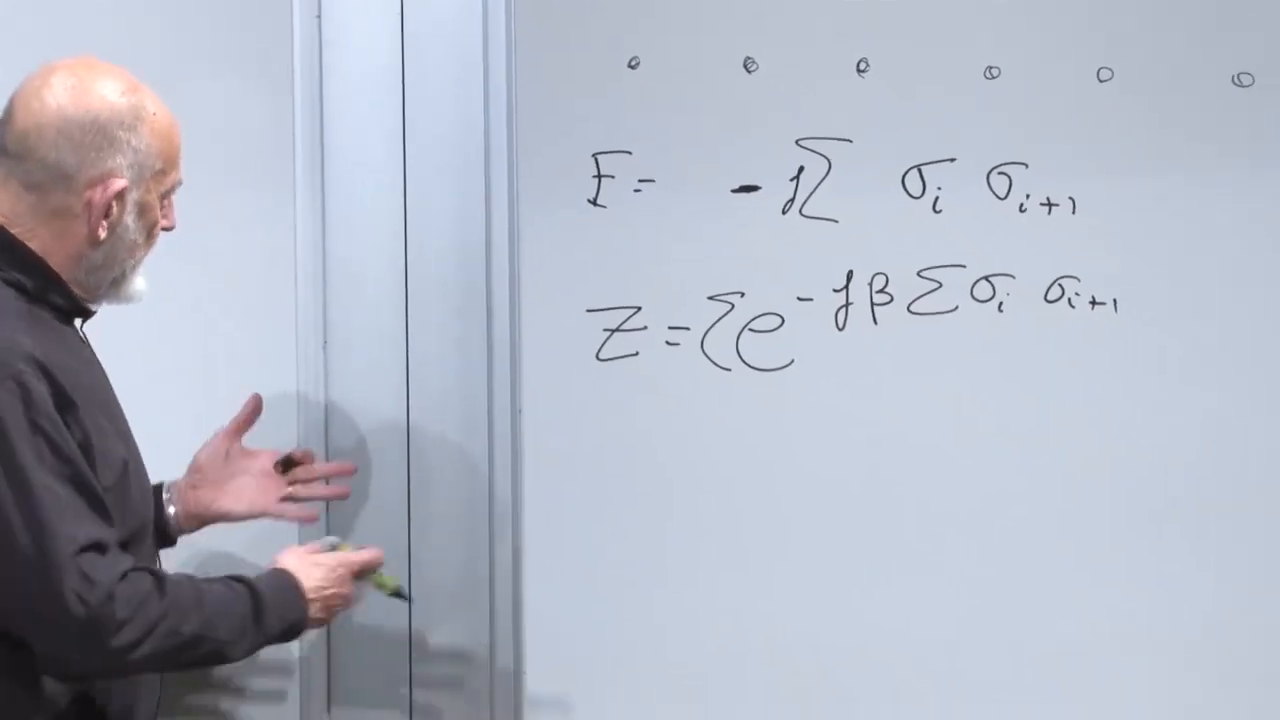
\includegraphics[width=0.80\textwidth]{lecture_09_figure_03.png}
\caption{開いた鎖のハミルトニアンとそのボルツマン和。}
\lectureframe{00:19:15}
\end{figure}

\(J\)を\(-J\)に変えると、交互に並ぶスピンが有利になる。開いた鎖、または偶数個の周期的鎖では、再定義
\begin{equation}
\widetilde{\sigma}_i=(-1)^i\sigma_i
\end{equation}
により反強磁性的な符号が強磁性的な符号に戻る。この区別は物理的であるが、一次元の分配関数の代数は同じである。奇数個の周期的鎖は、フラストレーションなしには交互に並べないため、よく知られた例外である。

\begin{classroomqa}
\audiencequestion{鎖のハミルトニアンに外部磁場はあるか？}
\lecturerresponse{まだない。式~\eqref{eq:ising-chain}には最近接結合のみが含まれている。一様な外部場は後に別の項\(-h\sum_i\sigma_i\)として加えられる。まさに、秩序状態が任意に小さなバイアスにどう応答するかを調べるためである。\lecturetimestamp{00:18:54--00:19:13}}
\end{classroomqa}

\subsection{相関関数としての記憶}

\(\sigma_i\)が上を向いていると分かっているとする。その情報は\(r\)個の結合を隔てたスピンに影響を及ぼすだろうか。診断法は
\begin{equation}
C(r)=\expect{\sigma_i\sigma_{i+r}}.
\end{equation}
である。\(C(r)\)が\(r\to\infty\)として非零の値に近づくなら、系は長距離の記憶を保持している。零に近づくなら、最初のスピンの効果はやがて消える。

伝言ゲームが正しい直観を与える。各人は次の人へ一つの二値記号を伝える。すべての伝達が完全なら、最初のビットはいつまでも生き残る。各段階にどんな非零の誤り確率があっても、伝達を繰り返すうちに元のメッセージはやがて失われる。零温度はイジング鎖の完全伝達の極限である。どんな正の温度でも、隣り合うスピンの間に時折の不一致が許される。

数値的な描像として、一回の伝達の忠実度が\(0.99\)であるとしよう。二回の完全な伝達は確率\(0.99^2=0.9801\)で起こり、段階が一つ増えるごとにさらに\(0.99\)の因子が掛かる。百段階では誤りはすでにありふれたものになり、一万段階では実用的な記憶は消える。イジング鎖はこの無誤り確率ではなく符号付きの忠実度の測度を用いるが、乗法的な損失は同じ考え方である。

この類推は、確率と相関を区別した後に厳密になる。\(p\)が隣り合うスピンが一致する確率なら、
\begin{equation}
\expect{\sigma_i\sigma_{i+1}}
=p-(1-p)=2p-1.
\end{equation}
である。したがって、結合から結合へと掛け合わされる量は過剰忠実度\(2p-1\)であり、\(p\)そのものではない。

\section{結合変数と厳密な分配関数}

決定的な変数変換は、個々のスピンではなく関係を記述することである。
\begin{equation}
\mu_i=\sigma_i\sigma_{i+1},
\qquad i=1,\ldots,N-1.
\label{eq:bond-variable}
\end{equation}
各結合変数は一致に対して\(+1\)、不一致に対して\(-1\)である。最初のスピンを固定すれば、結合がそれ以降のすべてのスピンを決める。
\begin{align}
\sigma_2&=\sigma_1\mu_1,\\
\sigma_3&=\sigma_1\mu_1\mu_2,\\
\sigma_{r+1}&=\sigma_1\prod_{k=1}^{r}\mu_k.
\end{align}
冗長性はない。データ\((\sigma_1,\mu_1,\ldots,\mu_{N-1})\)は\((\sigma_1,\ldots,\sigma_N)\)と等価である。

これらの変数ではエネルギーは単に
\begin{equation}
H=-J\sum_{i=1}^{N-1}\mu_i.
\end{equation}
である。相互作用するサイト変数は独立な結合変数になった。まず\(\sigma_1\)の二つの値について和をとると
\begin{align}
Z_N
&=2\sum_{\{\mu_i=\pm1\}}
\exp\left(\beta J\sum_{i=1}^{N-1}\mu_i\right)\\
&=2\prod_{i=1}^{N-1}
\left(\sum_{\mu_i=\pm1}e^{\beta J\mu_i}\right)\\
&=2\left[2\cosh(\beta J)\right]^{N-1}.
\label{eq:chain-partition}
\end{align}
が得られる。\(N-1\)個の因子があるのは、\(N\)個のサイトからなる開いた鎖が\(N-1\)個の結合をもつからである。

先頭の因子2は最初のスピンの大域的な選択である。それは\(\log Z_N\)に\(\log2\)だけ寄与し、一方、結合は\(N-1\)に比例する項を寄与する。この因子は厳密な有限サイズの数え上げには重要だが、\(N\to\infty\)として自由エネルギー密度からは消える。だからこそ板書はそれを実際に捨てることなく「大したことではない」と呼べたのである。

\begin{figure}[ht]
\centering
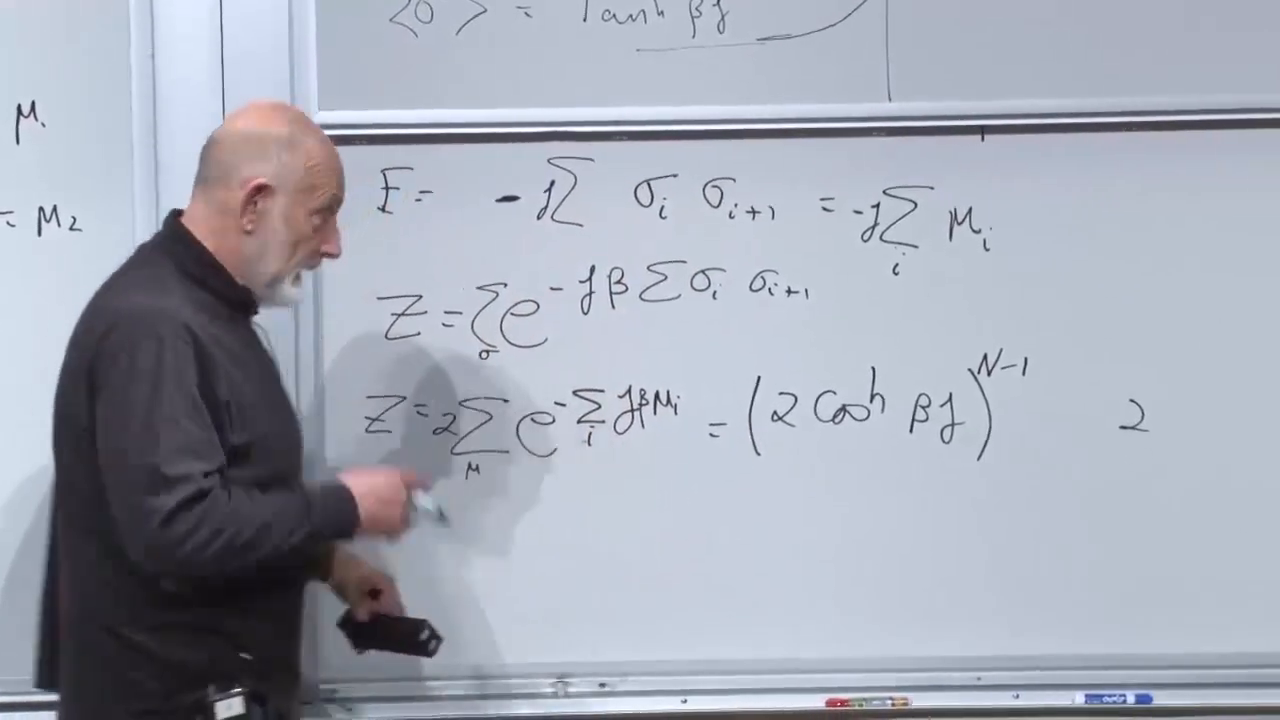
\includegraphics[width=0.82\textwidth]{lecture_09_figure_04.png}
\caption{独立な結合の和として書き直されたサイトのハミルトニアンと、その結果として因数分解された分配関数。}
\lectureframe{00:35:35}
\end{figure}

\begin{classroomqa}
\audiencequestion{最終的な答えが冪になったとき、指数の中の和はどこへ行ったのですか。}
\lecturerresponse{それは冪になる前に積になった。
\[
e^{\beta J\sum_i\mu_i}=\prod_i e^{\beta J\mu_i}.
\]
すべての結合配置にわたる和は、各結合に対する一つの二項の和に分離する。すべての因子が\(2\cosh(\beta J)\)であるから、積はその\((N-1)\)乗である。三つのスピンと二つの結合を書き下せば、因数分解は完全に明示的になる。\lecturetimestamp{00:33:25--00:35:36}}
\end{classroomqa}

これは単純な双対記述である。サイト上の結合した変数が、結合上の結合していない変数に置き換えられた。\emph{双対性}という語が適切なのは、同じ系が非常に異なって見える自由度をもつ二つの記述をもつからである。ここではそれは開いた一次元鎖に対する厳密な変数変換である。

格子の言葉では、元の変数は頂点に住み、新しい変数は辺に住む。最初のスピンの大域的な選択は、辺から頂点を再構成するために必要な唯一の余分なデータである。このサイトと結合の交換は、より高次元の統計力学ではるかに強力になるパターンのささやかな例である。

\subsection{最近接忠実度}

すべての結合は同じ分布をもち、
\begin{equation}
\begin{aligned}
\Pr(\mu=+1)&=\frac{e^{\beta J}}{2\cosh(\beta J)},\\
\Pr(\mu=-1)&=\frac{e^{-\beta J}}{2\cosh(\beta J)}.
\end{aligned}
\end{equation}
である。したがって、
\begin{equation}
\expect{\mu_i}
=\expect{\sigma_i\sigma_{i+1}}
=\tanh(\beta J).
\label{eq:nearest-correlation}
\end{equation}

\begin{figure}[ht]
\centering
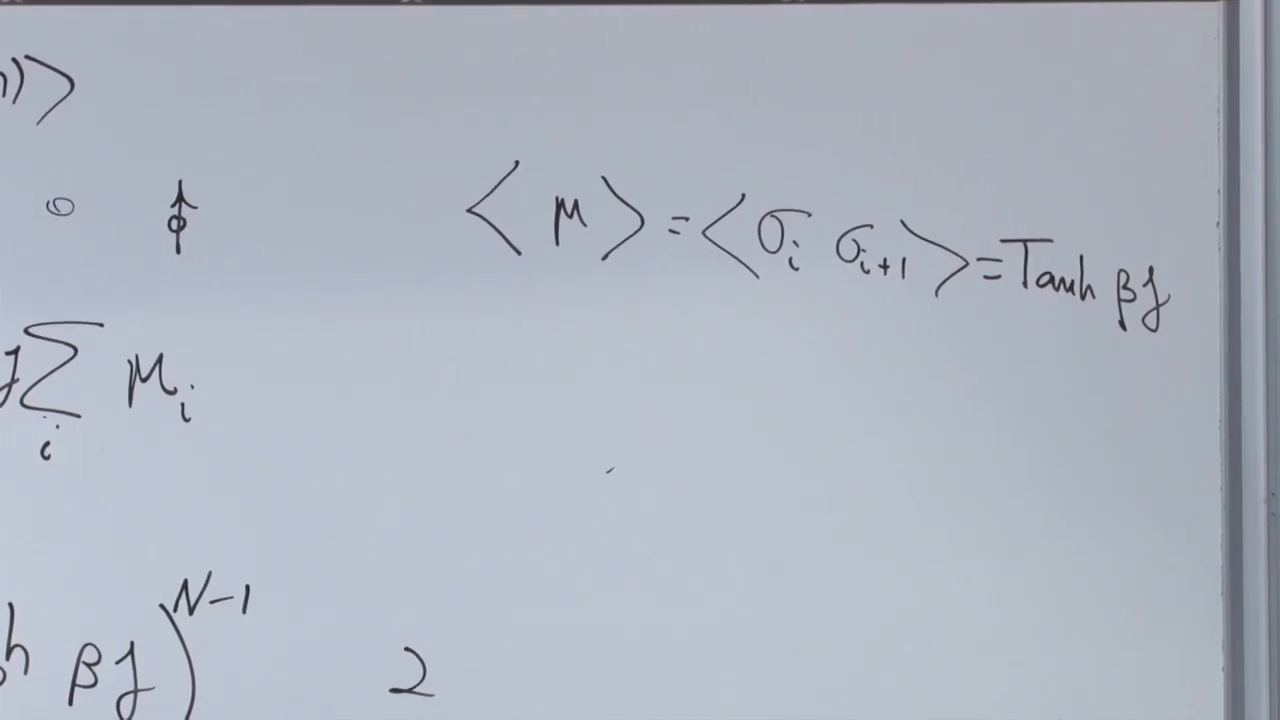
\includegraphics[width=0.80\textwidth]{lecture_09_figure_05.png}
\caption{平均結合変数として表された最近接相関。}
\lectureframe{00:36:52}
\end{figure}

したがって、隣り合うスピンが一致する確率は
\begin{equation}
p_{\rm same}
=\frac{1+\tanh(\beta J)}{2}.
\end{equation}
である。これは正の\(J\)で二分の一を超え、零温度で一に近づき、無限温度で二分の一になる。

\begin{classroomqa}
\audiencequestion{なぜ正の最近接相関は、スピンが反平行よりも平行を好むことを意味するのか。}
\lecturerresponse{\(J>0\)では、平行な結合のエネルギーは\(-J\)であり、反平行な結合のエネルギーは\(+J\)である。\(\expect{\mu}\)が正であることは、\(\mu=+1\)、すなわち平行がより頻繁に起こることを示している。実際の物質が強磁性または反強磁性の有効結合をもつかどうかは、その微視的な電子構造に依存する。ここでの符号の規約は強磁性体を記述している。\lecturetimestamp{00:43:45--00:44:48}}
\end{classroomqa}

\begin{classroomqa}
\audiencequestion{非常に高温ではこの相関はどうなるか。}
\lecturerresponse{\(T\to\infty\)のとき、\(\beta\to0\)かつ\(\tanh(\beta J)\to0\)となる。すると最近接のスピン同士でさえ互いについて何の情報ももたない。各スピンは実質的にランダムな推測である。\lecturetimestamp{00:46:42--00:47:20}}
\end{classroomqa}

\subsection{長距離相関}

\(r\)本だけ離れたスピンに対して、
\begin{align}
\sigma_i\sigma_{i+r}
&=\sigma_i
\left(\prod_{k=i+1}^{i+r-1}\sigma_k^2\right)
\sigma_{i+r}\\
&=(\sigma_i\sigma_{i+1})
(\sigma_{i+1}\sigma_{i+2})\cdots
(\sigma_{i+r-1}\sigma_{i+r})\\
&=\prod_{k=i}^{i+r-1}\mu_k.
\end{align}
\(\mu_k\)は独立であるから、
\begin{equation}
C(r)=\expect{\sigma_i\sigma_{i+r}}
=\left[\tanh(\beta J)\right]^r.
\label{eq:exact-correlation}
\end{equation}

\begin{figure}[ht]
\centering
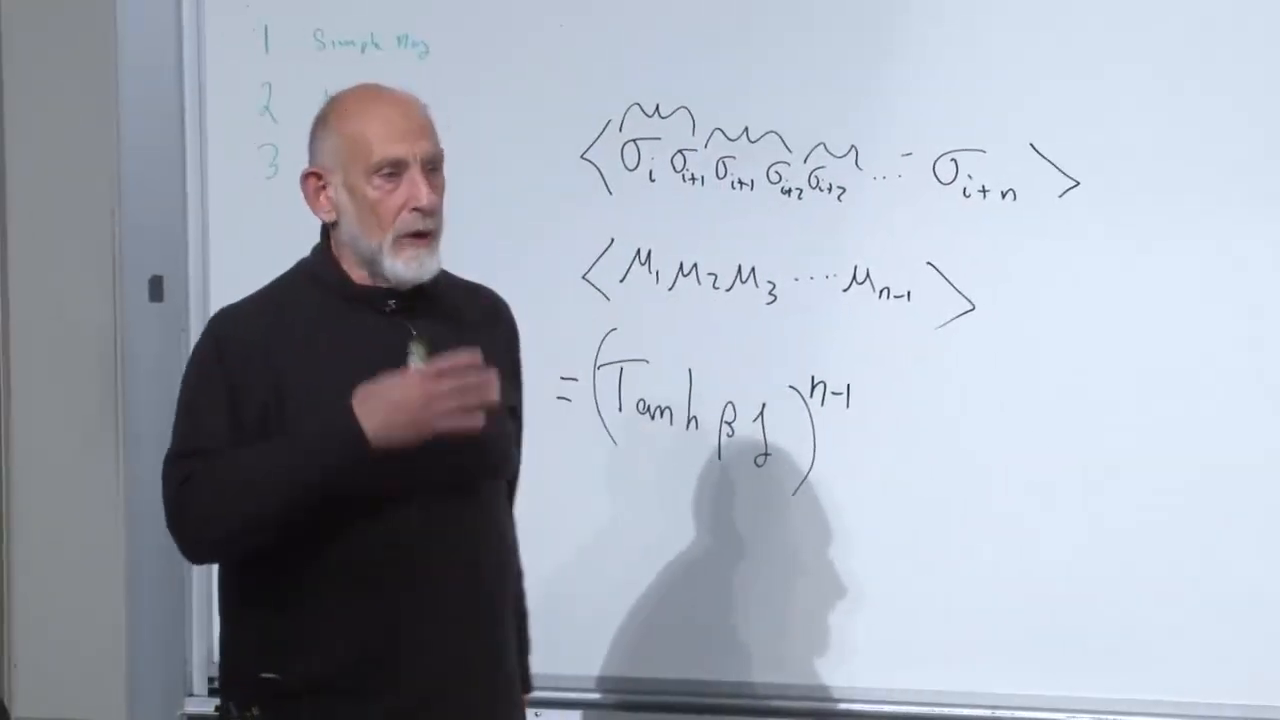
\includegraphics[width=0.80\textwidth]{lecture_09_figure_06.png}
\caption{中間の\(\sigma_k^2=1\)の因子が、遠方のスピンの積を独立な結合の積に変換する。}
\lectureframe{00:41:35}
\end{figure}

\begin{classroomqa}
\audiencequestion{相関関数には両端のスピンしか含まれていない。中間のスピンはどこから来たのか。}
\lecturerresponse{それらは1の因子として挿入されただけである: \(\sigma_k^2=1\)。隣接するコピーを対にすることで、端点の積が結合変数に変換される。結合変数こそ、その熱分布が因子分解する変数である。相関関数の値は変わっていない。\lecturetimestamp{00:41:41--00:42:26}}
\end{classroomqa}

すべての有限温度で、
\begin{equation}
0<\tanh(\beta J)<1,
\end{equation}
であるから、記憶は指数関数的に減衰する。
\begin{equation}
C(r)=e^{-r/\xi}
\end{equation}
と書くと、厳密な相関長
\begin{equation}
\xi^{-1}=-\log\!\left[\tanh(\beta J)\right].
\label{eq:correlation-length}
\end{equation}
が定義される。\(T=0\)においてのみ\(\xi\)は発散する。低いがゼロでない温度では、
\begin{equation}
\xi\simeq \frac{1}{2}e^{2\beta J},
\end{equation}
であるから、鎖は真の無限距離秩序をもつことなく、非常に長い平行な連なりを含むことができる。

したがって鎖は塊状に見える。上向きスピンの長い連なりがあり、次に切り替わり、下向きスピンの長い連なりがあり、さらに別の切り替わりがある。低温は、ドメイン壁が稀であるために連なりを長くするが、ドメイン壁を完全に排除するわけではない。磁化には、単に非常に大きいだけでなく、無限の記憶長が必要である。

\section{隣人が増えると問題がどう変わるか}

1次元では誤り訂正ができない。ある結合がその前の結合と一致しなくなると、次のスピンには、どちらの向きが意図されていたかを独立に告げる情報源がない。したがって鎖は、時折の切り替わりで隔てられた長い平行ドメインからなる。

正方格子では各サイトは4つの最近接サイトをもつ。立方格子では6つである。\(d\)次元超立方格子では、
\begin{equation}
z=2d
\end{equation}
個の最近接サイトをもつ。3つの一致するメッセージと1つの不一致メッセージを受け取るサイトは多数決に従うことができる。多数の隣人の環境は、冗長なメッセージが誤り訂正を可能にするのとほぼ同じ仕方で、孤立した誤りを抑圧する。

隣人が平均スピン\(m\)をもつなら、その和の平均は\(zm\)である。その通常の揺らぎは\(\sqrt{z}\)の程度であるから、\(m=0\)から離れると、相対揺らぎはおよそ
\begin{equation}
\frac{\sqrt{z}}{z|m|}
=\frac{1}{\sqrt{z}\,|m|}.
\end{equation}
とスケールする。これが、大きな配位数で平均場がもっともらしくなる理由である。また、\(m\)が小さい臨界点の近くで近似が最も信頼できなくなることも警告している。

記憶に残る格言が大数の直観を捉えている。100の独立な投票が同じ方向に誤ることは unlikely である。定量的な版は平方根則である。\(z\)個の変数におけるコヒーレントなバイアスは\(z\)に比例するが、ランダムな不一致は通常\(\sqrt{z}\)にしか比例しない。したがって次元を増やすことは、隣人の数だけでなく、その集団的メッセージの信頼性をも変える。

\begin{classroomqa}
\audiencequestion{3より高い次元は物理的な磁性体に対応するのか。}
\lecturerresponse{空間次元として直接対応するわけではない。大きな\(d\)は、各サイトが多くの隣人をもち、平均化が制御可能になる可解極限である。そこで機構が見えれば、それが物理的な次元にどこまで生き残るかを問うことができる。イジング模型では、平均場は厳密な2次元の答えを与えないが、2次元ですでに有限温度転移には十分である。\lecturetimestamp{00:52:32--00:53:50}}
\end{classroomqa}

\section{自己無撞着問題としての平均場}

一つのスピン\(\sigma_i\)に注目する。その\(z=2d\)個の最近接スピンとの相互作用は
\begin{equation}
E_i=-J\sigma_i\sum_{j\in{\rm nn}(i)}\sigma_j.
\label{eq:local-energy}
\end{equation}
である。
\begin{equation}
m=\expect{\sigma}
\end{equation}
をスピン当たりの一様磁化とする。平均場近似では、揺らぐ最近接スピンの和をその平均で置き換える：
\begin{equation}
\sum_{j\in{\rm nn}(i)}\sigma_j
\longrightarrow zm=2dm.
\end{equation}
このとき、注目したスピンの有効一スピンエネルギーは
\begin{equation}
E_i^{\rm MF}=-2dJm\,\sigma_i.
\label{eq:mean-field-energy}
\end{equation}
となる。

\begin{figure}[ht]
\centering
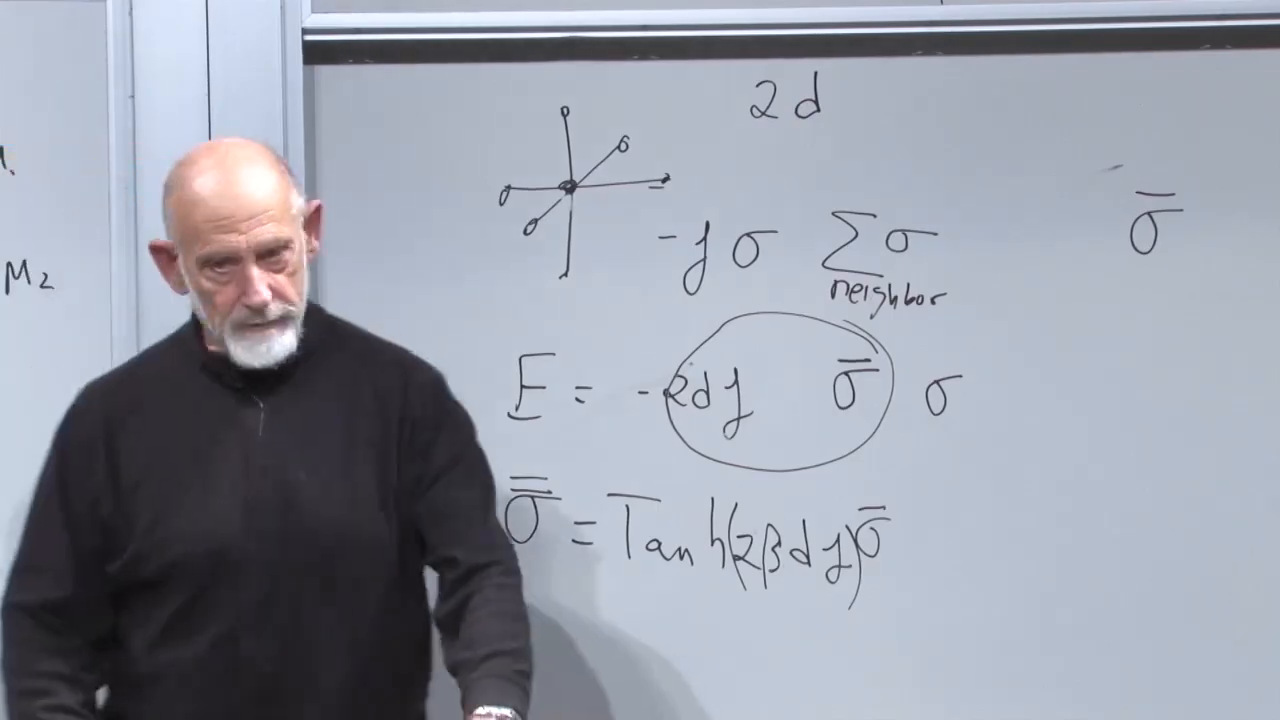
\includegraphics[width=0.82\textwidth]{lecture_09_figure_07.png}
\caption{選ばれたスピン、その\(2d\)個の最近接スピン、およびそれらの和を平均磁化で置き換えること。}
\lectureframe{01:00:30}
\end{figure}

一スピンの結果は、有効場\(2dJm\)を用いて再利用できる：
\begin{equation}
\expect{\sigma_i}_{\rm effective}
=\tanh(2\beta dJm).
\end{equation}
しかし、選ばれたサイトは特別ではない。並進不変性により、その平均は仮定された平均\(m\)に等しくなければならない。したがって
\begin{equation}
\boxed{m=\tanh(2\beta dJm)}.
\label{eq:self-consistency}
\end{equation}
これが、平均場が自己無撞着場近似とも呼ばれる理由である：有効場を生み出す磁化は、その場によって生み出される磁化に等しくなければならない。

\begin{classroomqa}
\audiencequestion{有効一スピンの答えには\(\beta\)の因子が欠けているのか？}
\lecturerresponse{それは存在しなければならない。指数関数や双曲線正接の引数は無次元であるから、有効エネルギー\(2dJm\)は\(2\beta dJm\)として現れる。\lecturetimestamp{01:00:13--01:00:27}}
\end{classroomqa}

\begin{classroomqa}
\audiencequestion{この方程式は、\(m\)がそれ自身に比例すると述べているだけなのか？}
\lecturerresponse{いいえ。未知の磁化は非線形関数の内部に現れる：
\[
m=\tanh(2\beta dJm).
\]
これは陰方程式であり、温度に応じて一つまたは複数の解を持ちうる。\lecturetimestamp{01:02:12--01:02:42}}
\end{classroomqa}

\begin{classroomqa}
\audiencequestion{自己無撞着方程式は、高温または双曲線正接の小さな引数を仮定しているのか？}
\lecturerresponse{いいえ。方程式\(m=\tanh(2\beta dJm)\)は、すべての温度における完全な平均場方程式である。\(\tanh x\simeq x\)のような後の近似のみが小さな\(x\)を必要とし、それは臨界点近傍で、現れる解を特定したり展開したりするために用いられる。\lecturetimestamp{01:02:44--01:03:12}}
\end{classroomqa}

\begin{classroomqa}
\audiencequestion{上線の記法は、通常の山括弧による平均とは異なるのか？}
\lecturerresponse{いいえ。黒板で用いられるバーは、熱平均の略記である：\(\bar{\sigma}=\expect{\sigma}=m\)。\lecturetimestamp{01:03:19--01:03:42}}
\end{classroomqa}

\begin{classroomqa}
\audiencequestion{\(2d\)個のスピンはすべて最近接スピンなのか、またより長距離の結合も同様の効果を持つのか？}
\lecturerresponse{超立方格子上では、はい：\(d\)個の座標軸のそれぞれに沿って二つの最近接スピンが存在する。次近接およびより遠い結合は別の模型であり、一般にそれぞれ独自の強さを持つが、相互作用の範囲を広げることは有効配位数も増やし、平均場の推論をより正確にしうる。\lecturetimestamp{01:03:43--01:05:12}}
\end{classroomqa}

\section{相転移のグラフ化}

定義する
\begin{equation}
K=2\beta dJ,
\qquad
y=Km.
\end{equation}
すると式~\eqref{eq:self-consistency}は
\begin{equation}
\frac{y}{K}=\tanh y.
\label{eq:graph-equation}
\end{equation}
となる。右辺は固定されたシグモイドである。左辺は原点を通る傾き
\begin{equation}
\frac{1}{K}=\frac{T}{2dJ},
\end{equation}
の直線である。ここで\(k_{\rm B}=1\)。

高温では直線は急であり、\(\tanh y\)と\(y=0\)のみで交わる。低温では直線は緩やかであり、三つの交点が存在する：\(y=0\)および対称な対\(y=\pm y_0\)。閾値は、直線と\(\tanh y\)が原点で同じ傾きを持つときに生じる。\(\tanh'(0)=1\)であるから、
\begin{equation}
K_c=1,
\qquad
T_c^{\rm MF}=2dJ.
\label{eq:mean-field-tc}
\end{equation}
これが平均場臨界温度であり、低次元における厳密な答えではない。

仮定\(J>0\)は、隣接スピンが一致することを好むと言っている；それは\(+m\)を\(-m\)より選び出すものではない。外部場がゼロのとき、ハミルトニアンは大域的フリップ\(\sigma_i\mapsto-\sigma_i\)によって変わらないので、二つの非零交点は物理的に等価である。グラフの正の半分のみを選ぶことは便利な作図上の慣習であり、負の相を失うことではない。

\begin{figure}[ht]
\centering
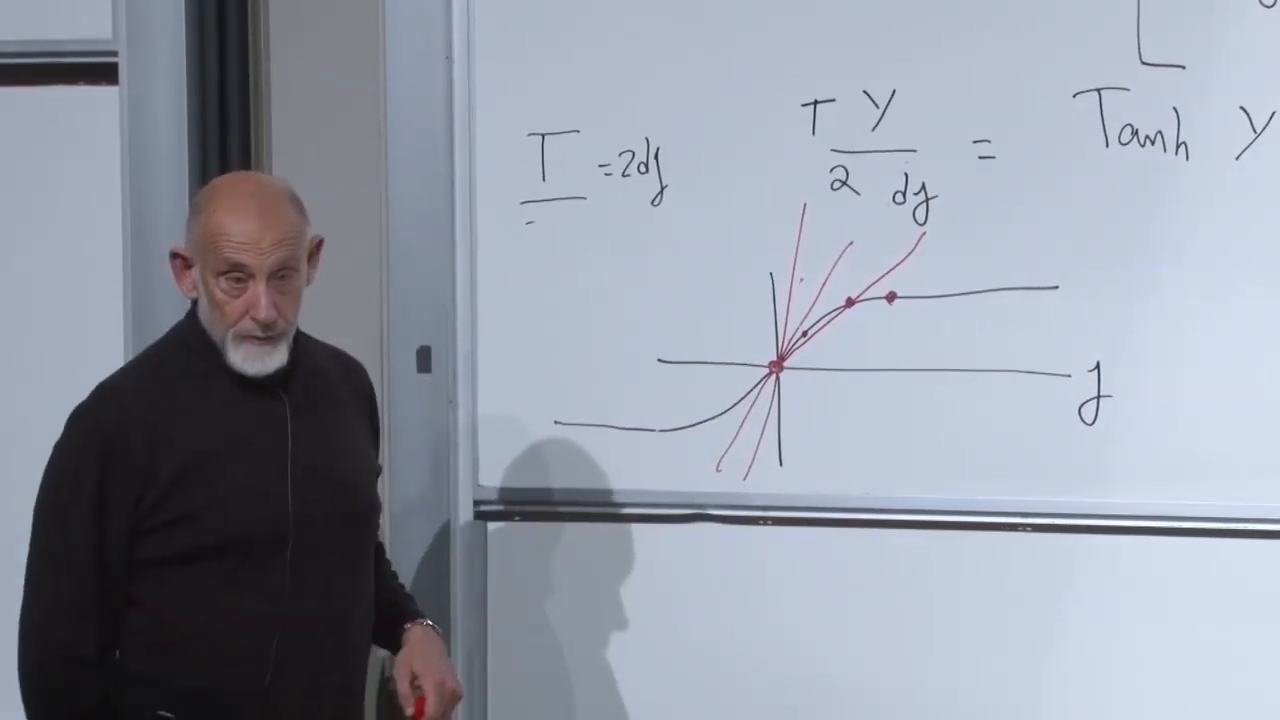
\includegraphics[width=0.82\textwidth]{lecture_09_figure_08.png}
\caption{直線族と\(\tanh y\)：高温での単一交点と低温での三つの交点。}
\lectureframe{01:11:50}
\end{figure}

\begin{figure}[ht]
\centering
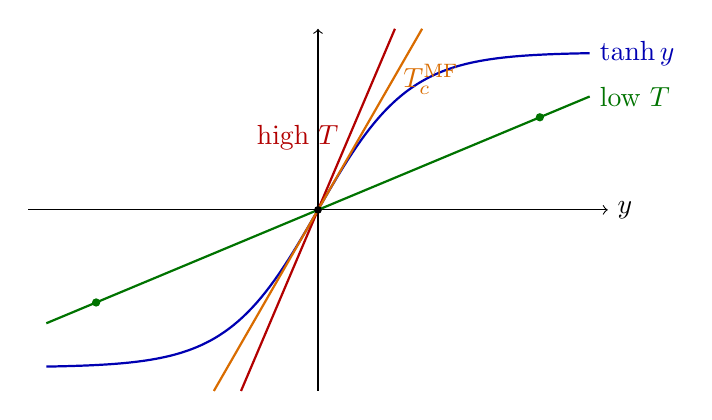
\begin{tikzpicture}[x=1.15cm,y=2.0cm]
\draw[->] (-3.2,0) -- (3.2,0) node[right] {$y$};
\draw[->] (0,-1.15) -- (0,1.15);
\draw[thick,blue!70!black,domain=-3:3,samples=120]
  plot (\x,{tanh(\x)}) node[right] {$\tanh y$};
\draw[thick,red!70!black] (-0.85,-1.15) -- (0.85,1.15)
  node[pos=0.70,left] {high \(T\)};
\draw[thick,orange!85!black] (-1.15,-1.15) -- (1.15,1.15)
  node[pos=0.86,right] {\(T_c^{\rm MF}\)};
\draw[thick,green!45!black] (-3,-0.72) -- (3,0.72)
  node[right] {low \(T\)};
\fill (0,0) circle (1.4pt);
\fill[green!45!black] (-2.45,-0.588) circle (1.5pt);
\fill[green!45!black] (2.45,0.588) circle (1.5pt);
\end{tikzpicture}
\caption{図形的自己無撞着論法の正規化された再構成。}
\end{figure}

非零の枝は連続的に現れる。転移近傍では、
\begin{equation}
\tanh(Km)=Km-\frac{(Km)^3}{3}+O(m^5).
\end{equation}
\(K>1\)に対して、小さな非零解は
\begin{equation}
m^2\simeq \frac{3(K-1)}{K^3}.
\end{equation}
を満たす。したがって平均場は、よく知られた平方根の立ち上がり\(m\propto(T_c-T)^{1/2}\)を予言する。

安定性の記述は、グラフがどのように描かれるかに依拠せずに行うこともできる。\(m\)に依存しない定数を除いて、一スピンあたりの平均場自由エネルギーは
\begin{equation}
f_{\rm MF}(m)
=dJm^2-\frac{1}{\beta}
\log\!\left[2\cosh(2\beta dJm)\right].
\label{eq:mf-free-energy}
\end{equation}
である。その停留条件は
\begin{equation}
\frac{\partial f_{\rm MF}}{\partial m}
=2dJ\left[m-\tanh(2\beta dJm)\right]=0.
\end{equation}
である。\(T_c^{\rm MF}\)より上では、\(m=0\)が最小である。それより下では、原点は局所的最大であり、二つの非零解は縮退した最小である。交点の幾何学と自由エネルギーの熱力学は同じことを述べている。

\begin{classroomqa}
\audiencequestion{解\(m=0\)は\(T_c^{\rm MF}\)の下で依然として交点である。なぜ非零の分枝が物理的でなければならないのか。}
\lecturerresponse{系を零温度から上昇させていくと、すでに磁化した分枝上に置かれる。より形式的には、平均場自由エネルギーは転移点以下で\(\pm m_0\)に極小をもち、一方\(m=0\)は極大となる。そのとき無限小の外部場が一方の極小を選び、見かけの曖昧さを取り除く。\lecturetimestamp{01:11:34--01:12:18}}
\end{classroomqa}

\section{なぜ一次元では平均場が破れるのか}

\(d=1\)を式~\eqref{eq:mean-field-tc}に代入すると、\(T=2J\)に転移があると予言することになり、厳密な一次元解と矛盾する。代数的に発散するものは何もない。この近似が破れるのは、二つの隣接スピンが大きな統計的浴ではないからであり、また一次元のドメイン壁が例外的なエントロピーを担うからである。

すべて上向きの状態から始める。壊れた結合はそのエネルギーを\(-J\)から\(+J\)へ変えるので、壊れた結合一つあたりのコストは
\begin{equation}
\Delta E_{\rm bond}=2J.
\end{equation}
である。正方格子上では、反転したスピン一つが四つの結合を壊し、\(8J\)のコストがかかる。隣接する反転スピン二つは六つの壊れた結合からなる周囲長をもち、\(12J\)のコストがかかるのに対し、遠く離れた反転二つは八つの結合を壊し、\(16J\)のコストがかかる。

\begin{figure}[ht]
\centering
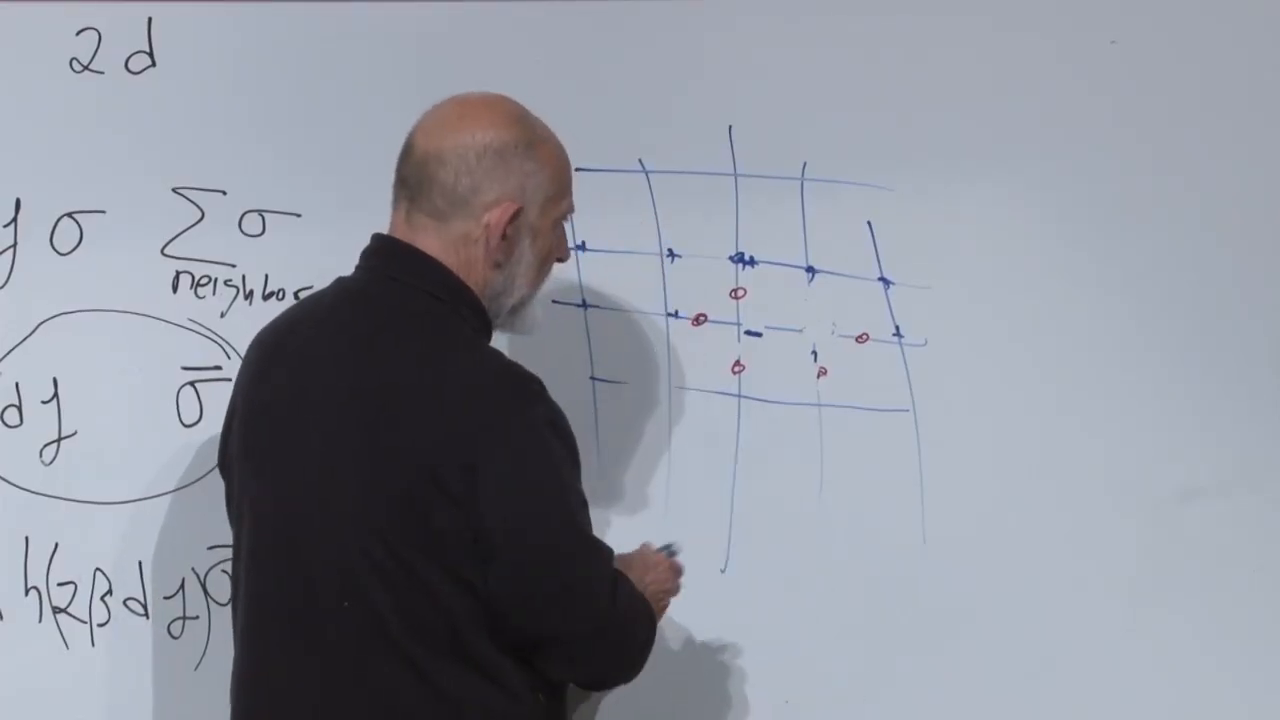
\includegraphics[width=0.82\textwidth]{lecture_09_figure_09.png}
\caption{正方格子上の隣接する反転スピン二つ。それらの共有結合は満たされており、六結合の境界が残る。}
\lectureframe{01:17:30}
\end{figure}

したがって二次元では、コンパクトな反転液滴はその境界長に比例するエネルギーを支払う：
\begin{equation}
\Delta E_{\rm 2d}=2J\,|\partial D|.
\end{equation}
液滴を成長させると、一般にその境界も成長する。

一次元は異なる。連続した反転ブロックは、どれほど長くても二つのドメイン壁しかもたない：
\begin{equation}
\Delta E_{\rm 1d}=2(2J)=4J.
\label{eq:one-d-domain-cost}
\end{equation}

\begin{figure}[ht]
\centering
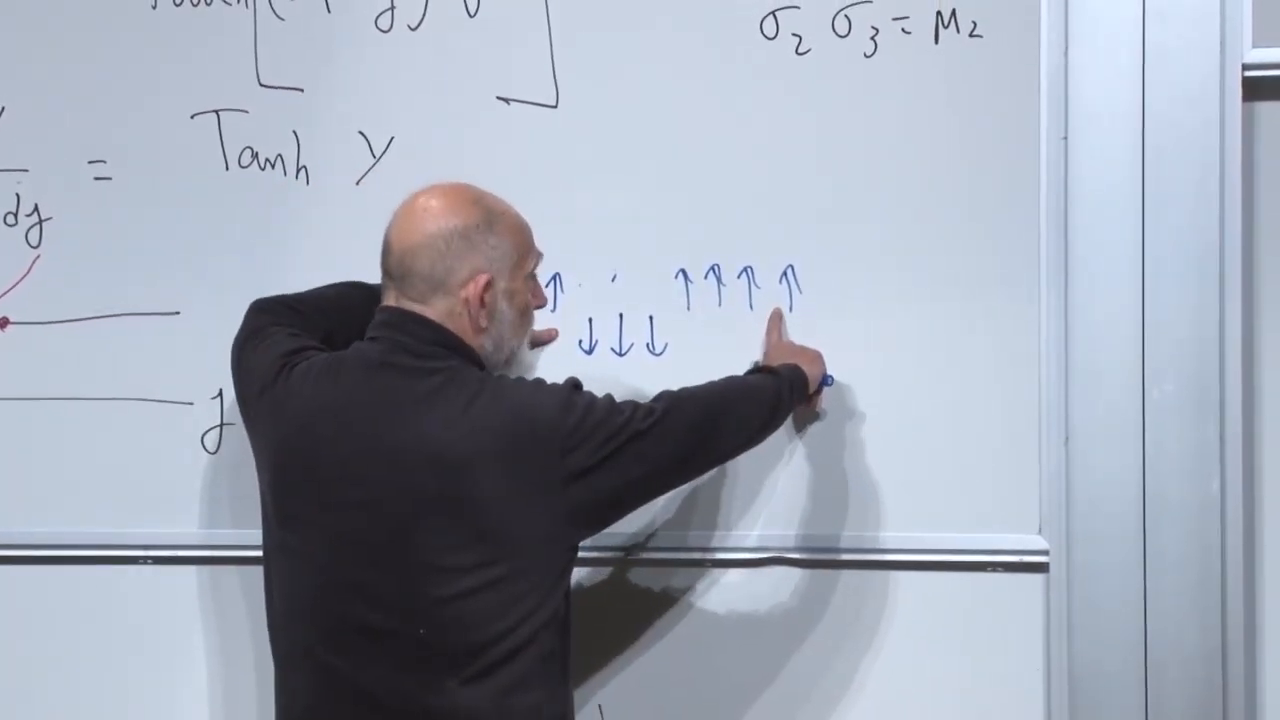
\includegraphics[width=0.82\textwidth]{lecture_09_figure_10.png}
\caption{一次元における長い反転ブロックは、二つのドメイン壁だけに囲まれている。}
\lectureframe{01:19:10}
\end{figure}

\(N\)サイトの鎖において、そのようなブロックの二つの壁を選ぶ方法は\(N^2\)の程度ある。それらのエネルギーは壁間の間隔とともに成長しない。任意の正の温度で、したがってエントロピーは任意に大きな反転ドメインを供給する。二次元では、境界エネルギーは十分低い温度で輪郭のエントロピーを打ち負かすことができる。このエネルギーとエントロピーの競合は、\(d=1\)と\(d=2\)を同じ係数の異なる数値として扱うとき、平均場が見ることのできない幾何学的事実である。

\begin{classroomqa}
\audiencequestion{二つの壁の一定コストは、反転スピンが隣接していることを要求するのか。}
\lecturerresponse{はい。この主張は一つの連続した反転ブロックに関するものである。反転スピンがいくつかの分離したブロックを形成するなら、各ブロックは二つの追加のドメイン壁を導入する。重要な点は、単一のブロックが二つの壁だけを保ちながら任意に長くなりうることである。\lecturetimestamp{01:18:32--01:18:40}}
\end{classroomqa}

\begin{classroomqa}
\audiencequestion{平均場方程式自体は\(d=1\)と\(d=2\)の間に定性的な区別を示さないように見える。それが問題なのか。}
\lecturerresponse{まさにその通りである。平均場はすべての正の\(d\)に対して転移を予言するので、一次元では定性的に誤っている。その導出は多数の弱く揺らぐ隣接スピンを仮定し、ドメイン壁の幾何学を捨て去った。一次元の場合を決めるのは、平均場の代入\(d=1\)ではなく、厳密な結合解である。\lecturetimestamp{01:19:44--01:20:28}}
\end{classroomqa}

\section{外部場が相を選ぶ}

\(h>0\)が\(\sigma=+1\)を好むという規約で、一様な場\(h\)を加える：
\begin{equation}
H=-J\sum_{\langle ij\rangle}\sigma_i\sigma_j
-h\sum_i\sigma_i.
\label{eq:ising-with-field}
\end{equation}
選ばれた一つのスピンの平均場エネルギーは
\begin{equation}
E_i^{\rm MF}=-(2dJm+h)\sigma_i,
\end{equation}
であり、自己無撞着方程式は
\begin{equation}
\boxed{m=\tanh\!\left[\beta(2dJm+h)\right]}.
\label{eq:self-consistency-field}
\end{equation}
となる。\(K=2\beta dJ\)および\(y=Km\)とすると、
\begin{equation}
\frac{y}{K}=\tanh(y+\beta h).
\label{eq:shifted-graph}
\end{equation}

\begin{figure}[ht]
\centering
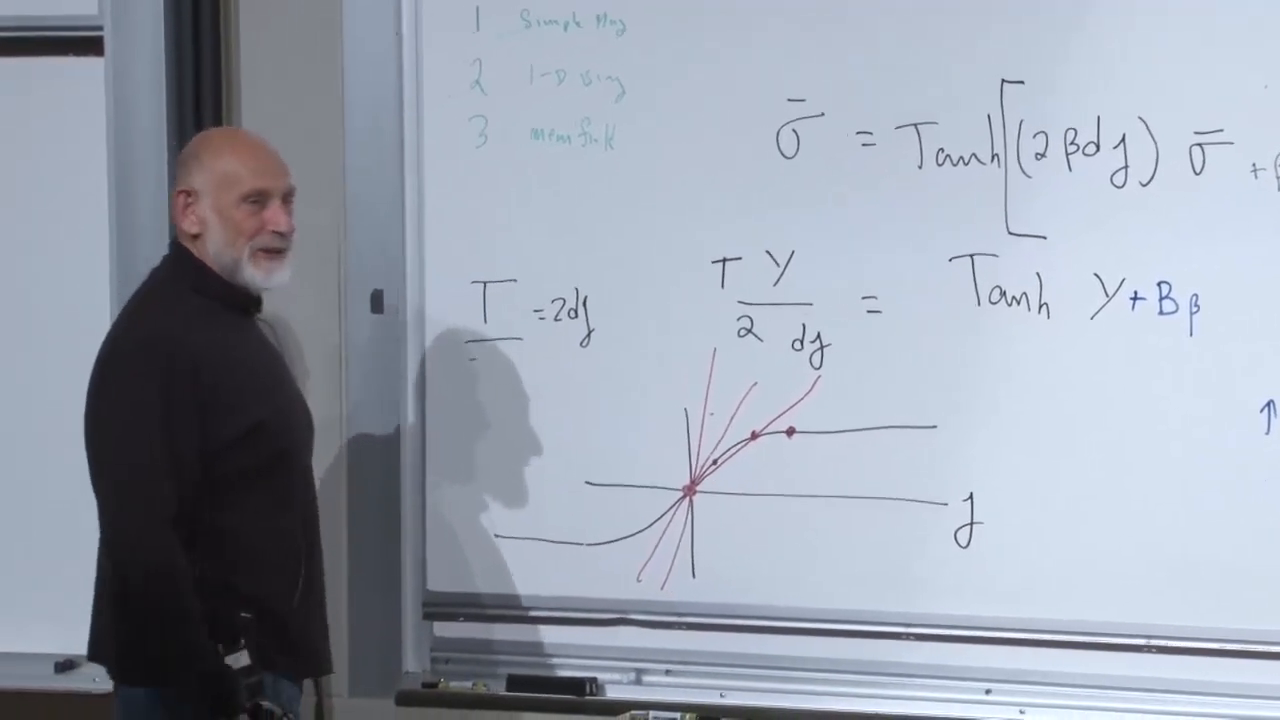
\includegraphics[width=0.82\textwidth]{lecture_09_figure_11.png}
\caption{自己無撞着方程式に加えられた外部場の項と、それに対応する平行移動した図式構成。}
\lectureframe{01:26:20}
\end{figure}

\begin{classroomqa}
\audiencequestion{なぜ場は双曲線正接の内部にのみ加えられるのか。左辺も変えるべきではないのか。}
\lecturerresponse{左辺は仮定された磁化\(m\)、あるいは同等に\(y/K\)である。右辺は全有効場\(2dJm+h\)中のスピンに対して計算された磁化である。自己無撞着性はそれら二つの量を等しく置く。\(y=Km\)を定義として固定しておくと、新しい項は引数\(\tanh(y+\beta h)\)の中にのみ入る。\lecturetimestamp{01:23:46--01:26:18}}
\end{classroomqa}

\begin{classroomqa}
\audiencequestion{同じ図式的変化は、\(\tanh\)曲線をずらすのではなく直線を動かすことによって記述できるか。}
\lecturerresponse{はい。\(\tanh y\)を固定したまま、直線が非零の切片をもつように方程式を書き直せばよい。交点は同一である。二つの記述は、方程式のどちら側を固定されたグラフとして選ぶかだけが異なる。\lecturetimestamp{01:35:07--01:36:26}}
\end{classroomqa}

\(h\neq0\)では、もはや原点は解ではない。\(T_c^{\rm MF}\)より下では、任意に小さい正の磁場が正の枝を選び、負の磁場が負の枝を選ぶ。

\begin{figure}[ht]
\centering
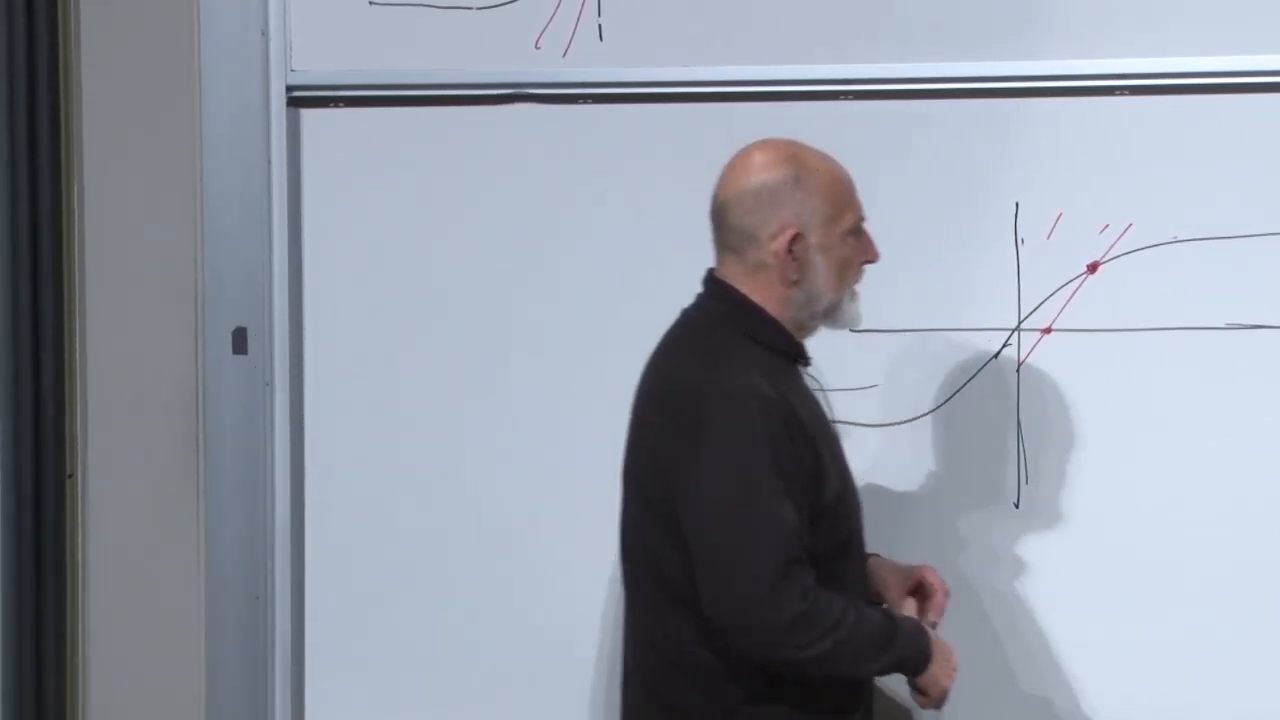
\includegraphics[width=0.82\textwidth]{lecture_09_figure_12.png}
\caption{弱い磁場は対称な交点を取り除き、磁化した一方の枝を選ぶ。}
\lectureframe{01:36:22}
\end{figure}

正確な記述には極限の順序が必要である。ちょうど\(h=0\)における有限系はスピン反転対称性をもつため、完全な平衡集団では\(\expect{m}=0\)である。自発磁化は
\begin{equation}
m_{\rm sp}
=\lim_{h\to0^+}\lim_{N\to\infty}\expect{m}_{N,h},
\end{equation}
であり、熱力学極限を先に取る。微小磁場の符号を逆にすると\(-m_{\rm sp}\)となる。全磁場エネルギーの差は\(Nh\)に比例するので、巨視的な試料ではごく小さな磁場でも決定的になる。

対応する自由エネルギーは傾きを可視化する：
\begin{equation}
f_{\rm MF}(m;h)
=dJm^2-\frac{1}{\beta}
\log\!\left[2\cosh\!\left(\beta(2dJm+h)\right)\right].
\end{equation}
\(h=0\)では二つの井戸は同じ深さである。正の\(h\)は正の\(m\)の井戸を下げ、負の\(m\)の井戸を上げる。スピン当たりの摂動はごく小さくても、\(N\)を掛けた全体的な選好は巨視的である。

\begin{classroomqa}
\audiencequestion{外部磁場が存在し続けるなら、磁化は本当に自発的なのか。}
\lecturerresponse{磁場は枝を選ぶためにのみ用いられる。\(T<T_c\)を固定し、系を無限大にしてから\(h\to0^+\)とする。選別磁場が消えても磁化は有限のままである。極限の符号を逆にすると反対の相が選ばれる。\lecturetimestamp{01:33:15--01:34:18}}
\end{classroomqa}

\begin{classroomqa}
\audiencequestion{転移より下で、平均ゼロの解は実際に不可能なのか、それとも単に不安定なだけなのか。}
\lecturerresponse{ちょうど磁場ゼロでは、二つの配向に等しい重みを与える対称な有限体積集団は可能であり、平均はゼロである。失敗するのは、単一の巨視的相としてのその安定性である。任意に小さい磁場が示量的なエネルギー均衡を変え、一方の配向を選ぶ。熱力学極限の後、選ばれた磁化は磁場を取り除いても生き残る。\lecturetimestamp{01:34:25--01:35:06}}
\end{classroomqa}

\begin{classroomqa}
\audiencequestion{無限温度で磁場に偏った解はどうなるのか。}
\lecturerresponse{固定された有限の\(h\)に対し、\(K=2\beta dJ\)と\(\beta h\)はともに\(T\to\infty\)で消える。式~\eqref{eq:self-consistency-field}はそのとき\(m\to0\)を与える。弱い磁場は低温の枝を選ぶが、無限の熱的攪乱に抗して秩序を維持することはできない。\lecturetimestamp{01:27:39--01:29:51}}
\end{classroomqa}

\begin{classroomqa}
\audiencequestion{温度とグラフのずれを同時に変えるとき、交点がどこへ行くかをどう確かめられるのか。}
\lecturerresponse{陰伏方程式は動くスケッチより安全である。低温で正の\(h\)では、その安定解は\(m=+1\)に近づく。高温では、正接の展開により
\[
m\simeq \beta(2dJm+h)
\quad\Longrightarrow\quad
m\simeq \frac{\beta h}{1-2\beta dJ},
\]
が得られ、これは\(\beta\to0\)でゼロに近づく。したがって安定枝は、整列した低温極限を弱く分極した高温極限へつなぎ、転移より下で不安定な原点にとどまることはない。\lecturetimestamp{01:29:53--01:33:04}}
\end{classroomqa}

\section{磁気反転は別の問題である}

\begin{classroomqa}
\audiencequestion{地球の磁場を反転させるものは何か。}
\lecturerresponse{その問いは平衡イジング模型の範囲外である。地球の主磁場はジオダイナモによって生成される。外核における電気伝導性流体の対流と回転が電流と磁場を維持する。反転はその非線形ダイナモの不規則な再編成であり、固体鉄における単純な強磁性ドメインの反転ではない。その詳細なタイミングは一つの平衡秩序変数では捉えられないので、ここでの正直な答えは、イジング計算は引き金を説明しないというものである。有用な関連は一般的なものに限られる。すなわち、二つの反対の大規模配向をもつ系はそれらの間で不安定性を起こしうる。\footnote{\href{https://science.nasa.gov/science-research/earth-science/earths-magnetosphere-protecting-our-planet-from-harmful-space-energy/}{ジオダイナモに関するNASAの概説}と\href{https://www.usgs.gov/programs/geomagnetism/introduction-geomagnetism}{地磁気に関するUSGSの入門}を参照。} \lecturetimestamp{01:38:39--01:40:32}}
\end{classroomqa}

厳密な鎖と平均場格子は今や二つの際立って異なる答えを与える。一次元では、
\begin{equation}
\expect{\sigma_i\sigma_{i+r}}
=\left[\tanh(\beta J)\right]^r
\longrightarrow0
\qquad (T>0),
\end{equation}
なぜなら有限エネルギーのドメイン壁が任意に長い反転区間を分離できるからである。多数の隣接スピンがある場合、自己無撞着場は代わりに
\begin{equation}
T_c^{\rm MF}=2dJ.
\end{equation}
より下で安定な非ゼロ解を許す。この対比は単に代数的なものではない。それは幾何、エネルギー、エントロピー、冗長性の間の競合である。すなわち、誤りが自由に広がりうるか、周囲の格子がそれを訂正できるかどうかである。